\documentclass[amssymb,twocolumn,aps]{revtex4}

% allows special characters (including æøå)
\usepackage[utf8]{inputenc}
%\usepackage [norsk]{babel} %if you write norwegian
\usepackage[english]{babel}  %if you write english

\usepackage{physics,amssymb}  % mathematical symbols (physics imports amsmath)
\usepackage{graphicx}         % include graphics such as plots
\usepackage[table]{xcolor}
\usepackage{xcolor}           % set colors
\usepackage{hyperref}         % automagic cross-referencing 
\usepackage{float}			  % force placement of tables and figures


\begin{document}
	
\title{Project 1 \\
    \normalsize FYS-STK4155}
\date{\today}               
\author{Selma Beate Øvland}
\affiliation{University of Oslo}

\newpage
	
\begin{abstract}

We study polynomial regression on the noisy Runge function, comparing Ordinary Least Squares (OLS), Ridge, and Lasso. Features are standardized using only training data and the target is centered so the intercept is not penalized. Performance is evaluated with test MSE/R², and we also examine gradient-descent variants.

We find that OLS performs well at low degrees but overfits as degree increases (rising MSE). Ridge reduces error at higher degrees by shrinking coefficients; Lasso achieves comparable accuracy with sparser models and improved numerical stability. Using 10-fold cross-validation, the best OLS model is degree 8 (test MSE 0.010). For Ridge at fixed degree 10, the optimal $\lambda$ = 0.01 yields MSE 0.0094—about 22 percent lower than OLS at the same degree (0.012). Bootstrap analysis indicates Ridge slightly increases bias but more substantially lowers variance, reducing total error. Adaptive gradient methods (e.g., Adam) converge faster than fixed step sizes. Overall, cross-validation and regularization produce more robust models than plain OLS.

\end{abstract}


\maketitle

\section{Introduction}
A challenge in machine learning methods for regression is to obtain a reliable input-output relationship from data while at the same time controlling the model complexity to avoid poor generalization. While polynomials can approximate smooth functions well, high degree models are prone to numerical instability and overfitting when data is noisy or features are not properly scaled. For effective regression models we want to balance simplicity and flexibility to minimize the expected prediction error. This critical tension is summarized by the bias-variance trade-off. \cite{compfys39}. \\

A model with high bias suffers from underfitting, failing to capture the complexity of the true function. A model with high variance suffers from overfitting, meaning it has learnt the noise of the training data leading to poor generalization on unseen data \cite{compfys38}, \cite{hastie}. Our goal in this project is to explore methods that balance this trade-off, as shown in \ref{fig:biasvariance}. To obtain models that are both stable and accurate, we make use of regularization and resampling techniques. Especially for multicollinearity issues we benefit from Ridge and Lasso regression, as they introduce a penalty term to the MSE cost function forcing the model parameters towards smaller magnitude which reduce variance. \\

In the project we will use the Runge function

\begin{equation}
    f(x) = \frac{1}{1 + 25x^2}
\end{equation}

to create a synthetic dataset of evenly spaced data points. We use this function to study how fitting it with high-polynomials illustrates the issue with interpolation instability and overfitting, which is a known phenomena useful for studying regularization methods \cite{wikipedia-runge}. \\

We first look at fitting OLS up to degree 15 on the Runge function in part (a), where we evaluate the accuracy with MSE and $R^2$ vs degree. In part (b) we study the penalty term $\lambda$ and it's relationship to the polynomial degree again using MSE and $R^2$ analysis. In part (c-f) we replace the equations with gradient-based solvers and examine convergence under different step sizes. In part (g) we implement bootstrap to separate the error into bias and variance, to explore the effect polynomial degree and sample size will have. Part (h) implements k-fold cross-validation and compares these test errors to the bootstrap estimates. In the end, we will have a method for diagnosing underfitting and overfitting, and selecting polynomial degrees and penalty terms that work well, as shown in \ref{fig:heatmap}. 

\section{Theory and Methods}

\subsection{Theory}
\label{subsection:theory}
Regression analysis assumes that the output data can be represented by a continous function f(x) plus noise. In linear regression this function is approximated linearly with 

\begin{equation}
    \overline{y} = X \theta
\end{equation}
This is a supervised regression problem where we assume that the true data is generated from a noisy model expressed as: 

\begin{equation}
y = f(x)+\varepsilon
\end{equation}

where in this project the true signal f(x) is expressed as the Runge function:

\begin{equation}
    f(x) = \frac{1}{1 + 25x^2}
    \label{eq:runge}
\end{equation}

and $\varepsilon$ represents the random normal distributed noise. 

The input domain for x is [-1,1] with additive Gaussian noise. 
\subsubsection{Ordinary Least Squares (OLS)}

The standard approach for OLS is to minimize the Mean Squared Error (MSE) cost function $C (\theta)$: 

\begin{equation}
    \min_{\theta\in\mathbb{R}^p} \; C(\theta)
= \frac{1}{n}\,\lVert y - X\theta \rVert_2^2
\end{equation}

Minimizing this function analytically leads to the solution for optimal parameters $\hat{\theta}_{\text{OLS}}$

\begin{equation}
\hat{\theta}_{\text{OLS}} = (X^\top X)^{-1} X^\top y
\end{equation}

The OLS estimator is unbiased, meaning the expectation value $\mathbb{E}\!\left[\hat{\theta}_{\text{OLS}}\right]$ equals the true parameter value $\theta$. The existence of a solution to OLS depends on invertibility of the Hessian matrix $H=X^TX$. Problems can arise if the design matrix X is high dimensional or if its columns are linearly dependent (known as super-collinearity), potentially leading to a singular (non-invertible) $X^TX$ matrix. \\

To address the issues described above we can use regularized regression like Ridge and Lasso. They add a penalty term to the standard OLS cost function. \\

\subsubsection{Ridge regression ($L_2$ regularization)} 

Ridge regression adds an $L_2$ norm penalty to the OLS cost function, controlled by a hyperparameter $\lambda \ge 0$

\begin{equation}
\min_{\theta \in \mathbb{R}^p}
\quad
\frac{1}{n}\,\lVert y - X\theta \rVert_2^2
\;+\;
\lambda \lVert \theta \rVert_2^2
\end{equation}

We find the optimal Ridge parameters $\hat{\theta}_{\text{Ridge}}$ analytically: 

\begin{equation}
    \hat{\theta}_{\text{Ridge}}
= (X^\top X + \lambda I)^{-1} X^\top y
\end{equation}

Adding $\lambda I$ ensures the matrix $X^\top X + \lambda I)$ is invertible for finite $\lambda$, solving the singularity issues OLS regression can have. In contrast to OLS, the Ridge estimator is biased for any $\lambda \ge 0$, but we also reduce variance. \\

\subsubsection{Lasso regression ($L_1$ regularization)}

The $L_1$ term is classified as 

\begin{equation}
\min_{\theta \in \mathbb{R}^p}
\quad
\frac{1}{n}\,\lVert y - X\theta \rVert_2^2
\;+\;
\lambda \lVert \theta \rVert_1
\end{equation}

where $\lVert \theta \rVert_1 = \sum_{i=1}^p \lvert \theta_i \rvert$. \\

The Lasso cost function normally does not yield an analytical solution. We need to solve it numerically, typically with variants of gradient descent methods. A key difference between Lasso and Ridge, is that where Ridge shrinks some of the coefficiants towards zero, Lasso will reduce some of them entirely to zero. This means that where Ridge keeps all the coefficients, Lasso only keeps a subset of them. This can be an advantage if we want sparser models (and if the true signal is sparse), but Ridge has an advantage where the true signal is more dense and we have multicollinearity. Using Lasso in the wrong way can make it underfit and oversimplify. 

\subsubsection{Optimization algorithms}

\textit{4.1 Convergence and divergence} \\

The MSE cost function of both OLS and Ridge are convex functions, where for a convex function any local minimum is also a global minimum, guaranteeing that the Gradient Descent (GD) cost function is also a convex function if the learning rate is sufficiently small. \\

\textit{4.2 Gradient descent (GD), fixed learning rate $\eta$} \\

Plain GD iteratively updates the parameters $\theta$ by taking a step proportional to the negative gradient of the cost function $C(\theta)$: 

\begin{equation}
\theta_{k+1} \;=\; \theta_k \;-\; \eta \,\nabla_{\theta} C(\theta_k)
\end{equation}

Simply put, the step size is the same for every parameter. In ML models the full gradient $\nabla_{\theta} C(\theta)$ must be computed by summing over all datapoints in a dataset. Calculating this full gradient is computationally expensive when the datasets become large. \\ 

\textit{4.3 Stochastic gradient descent (SGD)} \\

With stochastic gradient descent the cost function $C(\theta)$ can be expressed as a sum over the individual losses $c_i(x_i,\theta)$ for N data points:

\begin{equation}
    C(\theta) = \frac{1}{N}\sum_{i=1}^{N} c_i(x_i,\theta)
\end{equation}

SGD introduces randomness and computational efficiency by approximating the full gradient $\nabla_{\theta} C(\theta)$ by summing over a subset of the data $B_k$: 

\begin{equation}
    \theta_{j+1}
= \theta_j - \eta_j \sum_{i \in B_k} \nabla_{\theta}\, c_i(x_i,\theta_j)
\end{equation}

\textit{4.4 Momentum and Adaptive Methods (AdaGrad, RMSProp, ADAM) } \\

These methods modify the learning rate $\eta$ to speed up convergence: 

\begin{itemize}
    \item Momentum: moving average over the gradient =?
    \item AdaGrad: Each parameter has its own step size. If the parameter sees big gradients, shrink the step size; and if it rarely changes, increase the step size larger. 
    \item RMSProp: Similar to AdaGrad but uses an exponential moving average of squared gradients, to avoid AdaGrad's learning rate goes to zero problems. 
    \item ADAM: Combines momentum and RMSProp. Tracks average gradient (momentum) and average squared gradient (RMSProp), then bias-correct them early on. It is fast and stable on noisy and complex data. 
\end{itemize}

\subsubsection{Evaluation metrics}

\textit{5.1 Mean squared error (MSE)} \\

MSE is the squared difference between the true values ($y_i$) and the model's predicted values ($\overline{y_i}$). It's squared to punish the big differences more than the small ones, and to avoid positives/negatives canceling each other out. The lower value the better (smaller error). \\

Its mathematical expression is 

\begin{equation}
    \text{MSE}(y, \tilde{y}) = \frac{1}{n} \sum_{i=0}^{n-1} (y_i - \tilde{y}_i)^2 
\end{equation}

It's best to use MSE to optimize and see absolute error size. MSE is sensitive to outliers. \\

\textit{5.2 $R^2$ score function} \\

The $R^2$ score function represents how much better your model is than just measuring the mean of the training data. It's represented as a quantile, where 1 equals perfect predictions and 0 means no better predictions than the mean, so a high value is better. Definition: 

\begin{equation}
    R^2 \;=\; 1 \;-\; \frac{\sum_{i=1}^n (y_i - \hat y_i)^2}{\sum_{i=1}^n (y_i - \bar y_{\text{train}})^2}
\end{equation}

We use the $R^2$ as a score for how good the fit of our model is. 

\subsubsection{Bias-Variance tradeoff}

The MSE can be decomposed into three fundamental components: 

\begin{equation}
    \mathbb{E}\!\big[(y-\tilde y)^2\big]
= \operatorname{Bias}^2[\tilde y]
+ \operatorname{Var}[\tilde y]
+ \sigma^2
\end{equation}

\begin{itemize}
    \item Bias squared ($\operatorname{Bias}^2[\tilde y]$): Represents the error due to simplifying assumptions in the model (e.g. modeling a complex non-linear function using a low-order polynomial). 
    \item Variance ($\operatorname{Var}[\tilde y]$): Measures how much the predicted values $\overline{y}$ changes over different training data sets. Highly flexible models usually have high variance. 
    \item Irreducible error ($\sigma^2$): The variance of the noise inherent in the data, which cannot be reduced by the model. 
\end{itemize}

The Bias-Variance trade off represents the relationship between a model's complexity (bias) and its sensitivity to the training data (variance). 
A simple model (low complexity) has high bias and low variance. 
A complex model (high flexibility) has low bias and high variance, adapting too closely to the noise in the training data. With Ridge and Lasso we introduce a small bias, but in return we achieve a greater reduction in variance, usually resulting in lower expected test error (MSE) than with OLS. 

\subsubsection{Generalization error estimators}

\subsubsubsection{Hold out}

Split the data randomly into training and test data sets. For each model complexity (polynomial degree or regularization factor $\lambda$) we first fit on train, then compute test and train MSE. As complexity increases, train MSE usually decreases, while test MSE will have a characteristic U-shape: high error from underfitting at low complexity, a good fit in the middle and overfitting at high complexity. This helps us choose the complexity that minimizes test MSE. Understanding the relationship between test errors, train errors and model complexity is fundamental to understanding the bias-variance trade-off. 

\subsubsubsection{Bootstrap}

We use our training dataset and re-draw samples from it (with replacement), several times. We then fit our model to the new datasets, to see how predictions change. For each test point we compute average prediction, variance, MSE, and squared bias. This tells us if our model is stable (low variance) or touchy (high variance) as we nudge the data. 

\subsubsubsection{K-fold Cross-Validation (CV)}

K-fold CV is a resampling technique designed to avoid issues where random splitting might lead to an unbalanced influence of certain samples on model building or evaluation. We split the data into K equal parts (or folds). For each setting (degree or regularization parameter) we train on K-1 fold, and evaluate on the left-out fold. We repeat this so every fold is the test set once. Average over the K-errors to get CV-MSE. This way we train and split more than just once, which helps if data is sparse. Using CV-MSE we can pick the best complexity and retrain with the chosen complexity.  

\subsubsection{Scaling, centering and data splitting}

Standardizing or rescaling data is crucial for numerical stability and model performance, especially if the design matrix X contains features on drastically different scales, which can happen if using high-degree polynomials (as columns with high polynomials would explode or vanish). Putting all features on a comparable scale avoids letting large-scale features dominate the $X^TX$ matrix. In Ridge or Lasso where we penalize the size of the coefficients, we need a comparable scale so the strength of the regularization parameter $\lambda$ has a consistent meaning across features. \\

We split the data into training and testing data. The purpose of the testing data is to simulate unseen data to evaluate a model's performance. It is important to split the data before doing any kind of standardization, as this keeps the test data "hidden" from the model. We only standardize the training data (this action let's the model "see" the data, which is why we don't do it on the test data). So after fitting the transformation parameters into the training data, we apply the fitted transformation to both the test and the training matrix. The test set must be transformed using the mean and standard deviation derived from the training set, and not itself. When we use K-fold CV, this principle extends to each fold. When using a fold as the test set, the standardization parameters must be calculated from the other folds (the K-1 folds). 

\subsection{Methods - Implementation}
\label{section:methods}

We will do a regression analysis by implementing stepwise the methods talked about in the Theory section for several polynomial degrees. Through all our tests we will use the Runge function \eqref{eq:runge}, and we will evaluate the methods using MSE and $R^2$. 


\subsubsection{Generating our data set and preprocessing}
 \label{subsec:data}

We study supervised regression of noisy observations 

\begin{equation}
    y = f(x) + \varepsilon, \qquad \varepsilon \sim \mathcal{N}(0,\sigma^2)
\end{equation}

where $f(x)$ is the Runge function \eqref{eq:runge} on [-1,1]. In our code, synthetic data is generated using the \texttt{make\_data(n=300, noise\_sd=0.3, seed=42)} function in data.py. It generates n input points uniformly spaced in the [-1,1] interval, evaluates Runge function at these points and adds Gaussian noise, where we end up with two arrays as the output, x (inputs) and y (targets). We fix the seed (\texttt{seed=42})throughout the calculations so the results are reproducible by using the function \texttt{ rng = np.random.default\_rng(seed) }.  \\

To give the model the flexibility to capture the shape of the curve, we expand each scalar input (x) into polynomial features using \texttt{build\_features(x,\ degree=p,\ include\_bias=False)} function, where the output is our design matrix. This produces columns with $x, x^2, x^3 .. x^p$ where include\_bias=False, means we omit the intercept column. Each column represents the complexity we have chosen for our model. We handle the intercept separately by centering the training targets and adding back the mean at prediction time. We do this because the intercept column contribute nothing to the standardizations, and we don't want Ridge/Lasso to penalize the intercept column. After, we split the dataset into train and test. The StandardScaler function is fitted on the training matrix, then after we scale both training and test matrix with the training mean and std. We also center the training targets by subtracting their training mean. This is the procedure for standardization we will use throughout the project, apart from when we implement k-fold CV, where we need to tweak our preprocessing procedure a little. We will go into detail about this later in this section. \\

\subsubsection{Ordinary Least Square (OLS) for the Runge function}
\label{subsec:ols}

We start with the simplest closed-form model; OLS. The OLS find a set of coefficients that matches the model's predictions as close as possible to the observed targets. In our implementation (\texttt{ fit\_ols}) we use the data set generated and preprocessing techniques described in Section \ref{subsec:data}, and solve the normal equations directly. The output from this are the parameters $\theta$. We calculate MSE and $R^2$ to evaluate the model's fit over the different polynomial degrees. We expect that the method will perform more poorly when increasing the polynomial degree. We also plot how the noise affects MSE and $R^2$. We expect a noise free model to work much better at higher polynomials than if we implement noise. We plot a noise-free and heavy noise scenario with MSE vs $R^2$ to see the effect. For the MSE we expect a U-shaped curve where the intermediate polynomial degrees are the best fit, and for the $R^2$ we expect the same effect, with an upside down U-shaped curve, where the low degrees and higher degrees are bad fits. We will also plot the parameters $\theta$ vs polynomial degree. We expect the parameter size to blow up as the degree increases. FIX \\

To make our model behave better with high-degree polynomials, we implement the $L_2$ norm penalty, Ridge regularization. \\

\subsubsection{Adding Ridge regression for the Runge function}

Data and polynomial features are produced by the same utilities explained in Section \ref{subsec:ols}, still using Runge as the target function. In \texttt{def fit\_ridge(X, y\_c, lam, n\_factor=True)} we add the $L_2$ term to the $X^TX$ term from OLS so this becomes $X^TX + \lambda I$ which reduce variance at the cost of small bias, but improving on MSE. We expect that the coefficients will shrink with the $L_2$ penalty. 

\subsection{Use of AI tools}
	
I used ChatGPT to help me make a plan for how to structure the code for this project. Before that, I started with part (a), wrote the code, then went to part (b) and realized I could reuse some code from part (a). I ended up with messy code without clear structure, with repeated variables and functions more times than needed. I wanted to separate the code and make it reusable for all parts of this project, and also for other projects/exercises later. So I uploaded the project description to ChatGPT and asked for a plan on how to organize the code (not the actual code). ChatGPT gave me a plan where I can make one Python file at a time (data, models, plotting, etc.), so I don’t have to think only in terms of part a, b, c, which was a bit overwhelming. This helps me keep the code cleaner and easier to reuse. \\
	
\section{Results and Discussion}\label{section:results} 

\subsection{Results}

\paragraph{Setup:}
Data from the Runge function
\[
f(x)=\frac{1}{1+25x^{2}}, \qquad x\in[-1,1],
\]
with additive Gaussian noise \(\varepsilon\sim\mathcal N(0,\sigma^{2})\).
For $\sigma = 0.3$  we construct polynomial features up to
degree \(p\le 15\), use a single train/test split, apply standardization
on the training data only, fit closed-form OLS on the centered target
\(y_{\text{train}}-\bar y_{\text{train}}\), and shift predictions back to the
original scale by adding \(\bar y_{\text{train}}\).

\subsubsection{Simplest CF method: Ordinary Least Square (OLS)}

We tested two different noise scenarios shown in figure \ref{fig:ols_vs_degree};  a noiseless dataset and a high noise dataset. For the noiseless scenario test MSE decreases monotonically with degree p, and approaches $\sim 0$. $R^2$ rises toward $\sim 1$. Higher degree improves fit. For a high noise dataset (sd=0.7) MSE is high and flattens out in particular areas, then rises sharply with complexity grade towards 1. $R^2$ fluctuates as well, but decreases sharply with complexity towards 0. 

\begin{figure}[H]
    \centering
    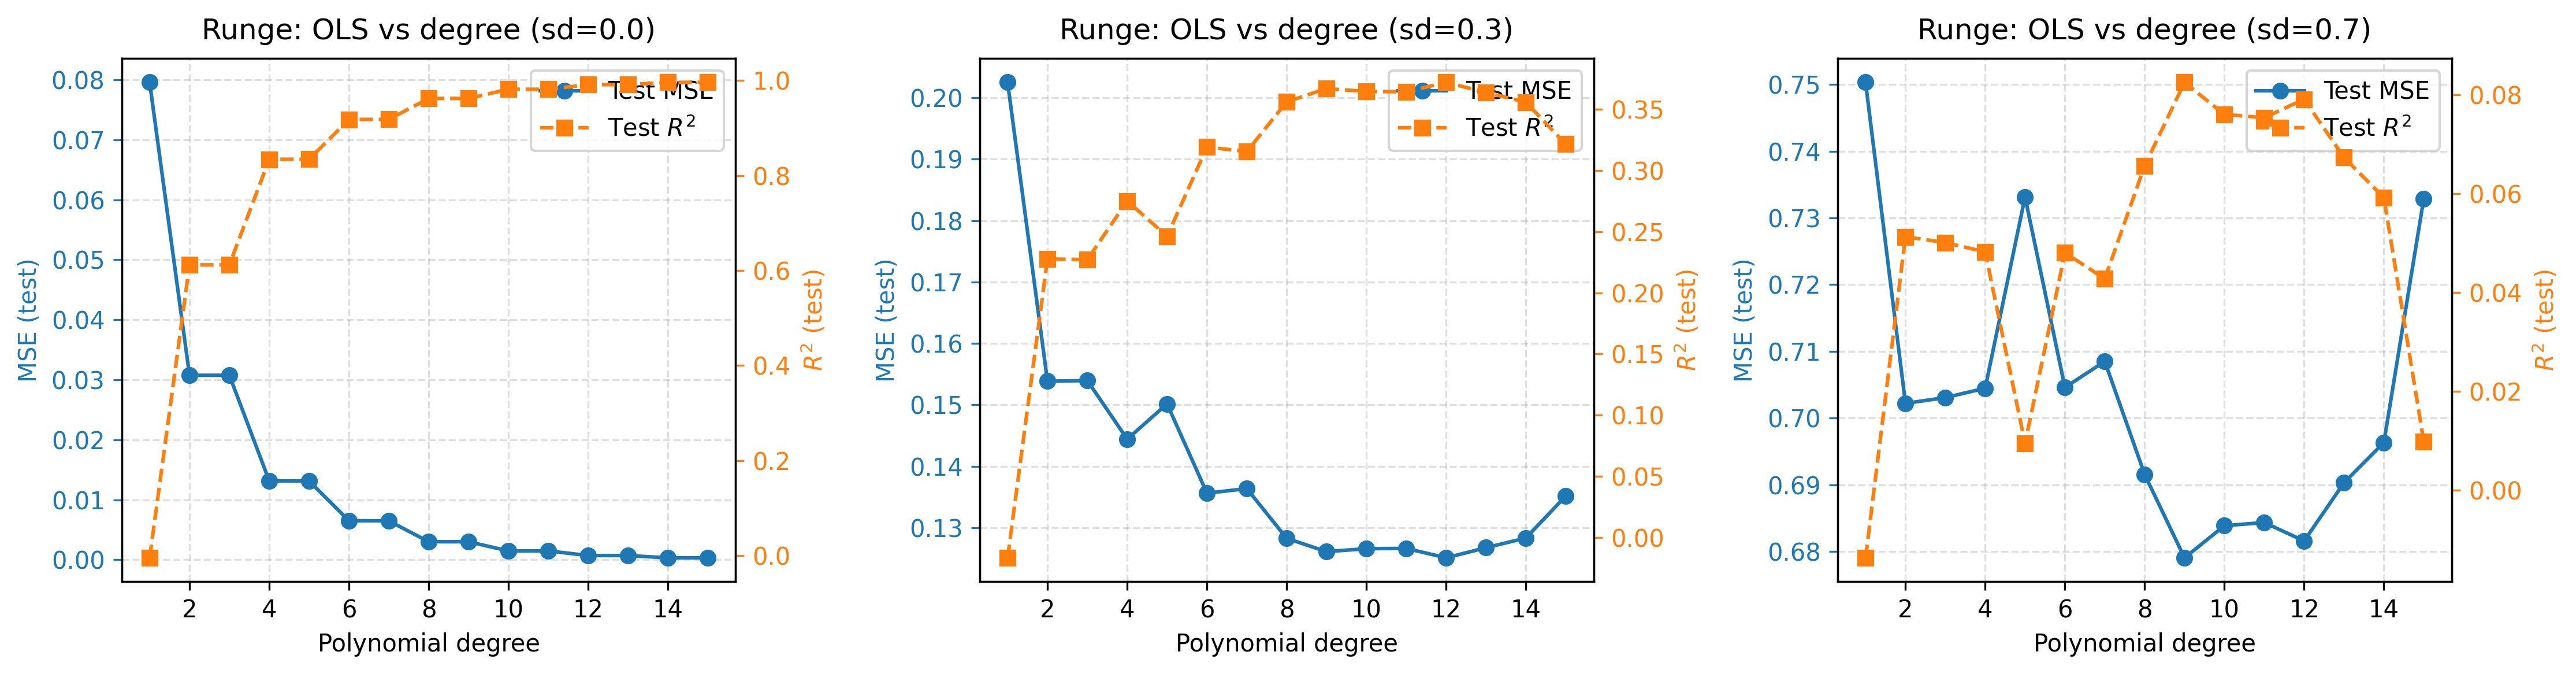
\includegraphics[width=1\linewidth]{Project-1/Figures/runge_ols_mse_r2_vs_degree.png}
    \caption{Test MSE vs polynomial degree, for different noise values.}
    \label{fig:ols_vs_degree}
\end{figure}

In figure \ref{fig:norms_vs_degree} and beyond, we have settled on a noise level between our two tests in figure \ref{fig:ols_vs_degree}, sd = 0.3, to replicate real data. In \ref{fig:norms_vs_degree} we plot the coefficent size vs degree p, and see that it remains modest at low to medium size p, then grows rapidly after p $\approx$ 12. 

\begin{figure}[H]
    \centering
    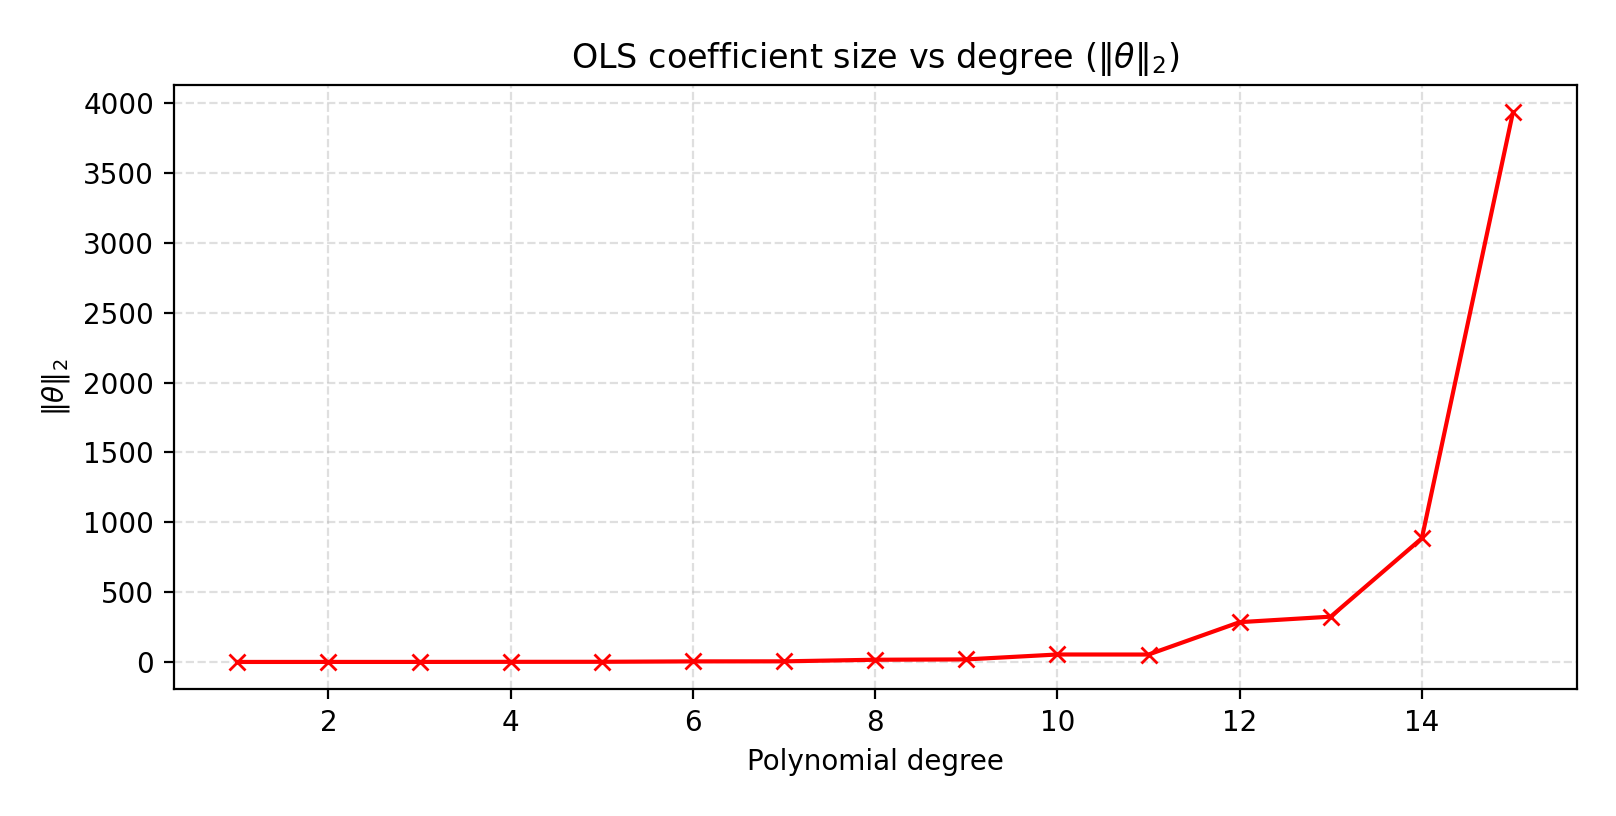
\includegraphics[width=1\linewidth]{Project-1/Figures/runge_ols_theta_norms_vs_degree.png}
    \caption{The figure shows the relationship between the $l_2$ norm of the OLS coefficients and the polynomial degree p.}
    \label{fig:norms_vs_degree}
\end{figure}

\subsubsection{Introducing the penalty term $\lambda$, CF Ridge regression}

In figure \ref{fig:ridge_mse_lambda} as the penalty term $\lambda$ increases from very small values, test MSE is smallest at around $\lambda \approx 10^{-4}-10^{-5}$ and then increases steadily from there. $R^2$ has its peak at the same region ($10^{-4}-10^{-5}$) and steadily decreases from there. In figure \ref{fig:ridge_theta_norms} the coefficient norm shrinks steadily as $\lambda$ increases. Shrinkage is most effective at $10^{-6}-10^{-3}$ then flattens out. 

\begin{figure}[H]
    \centering
    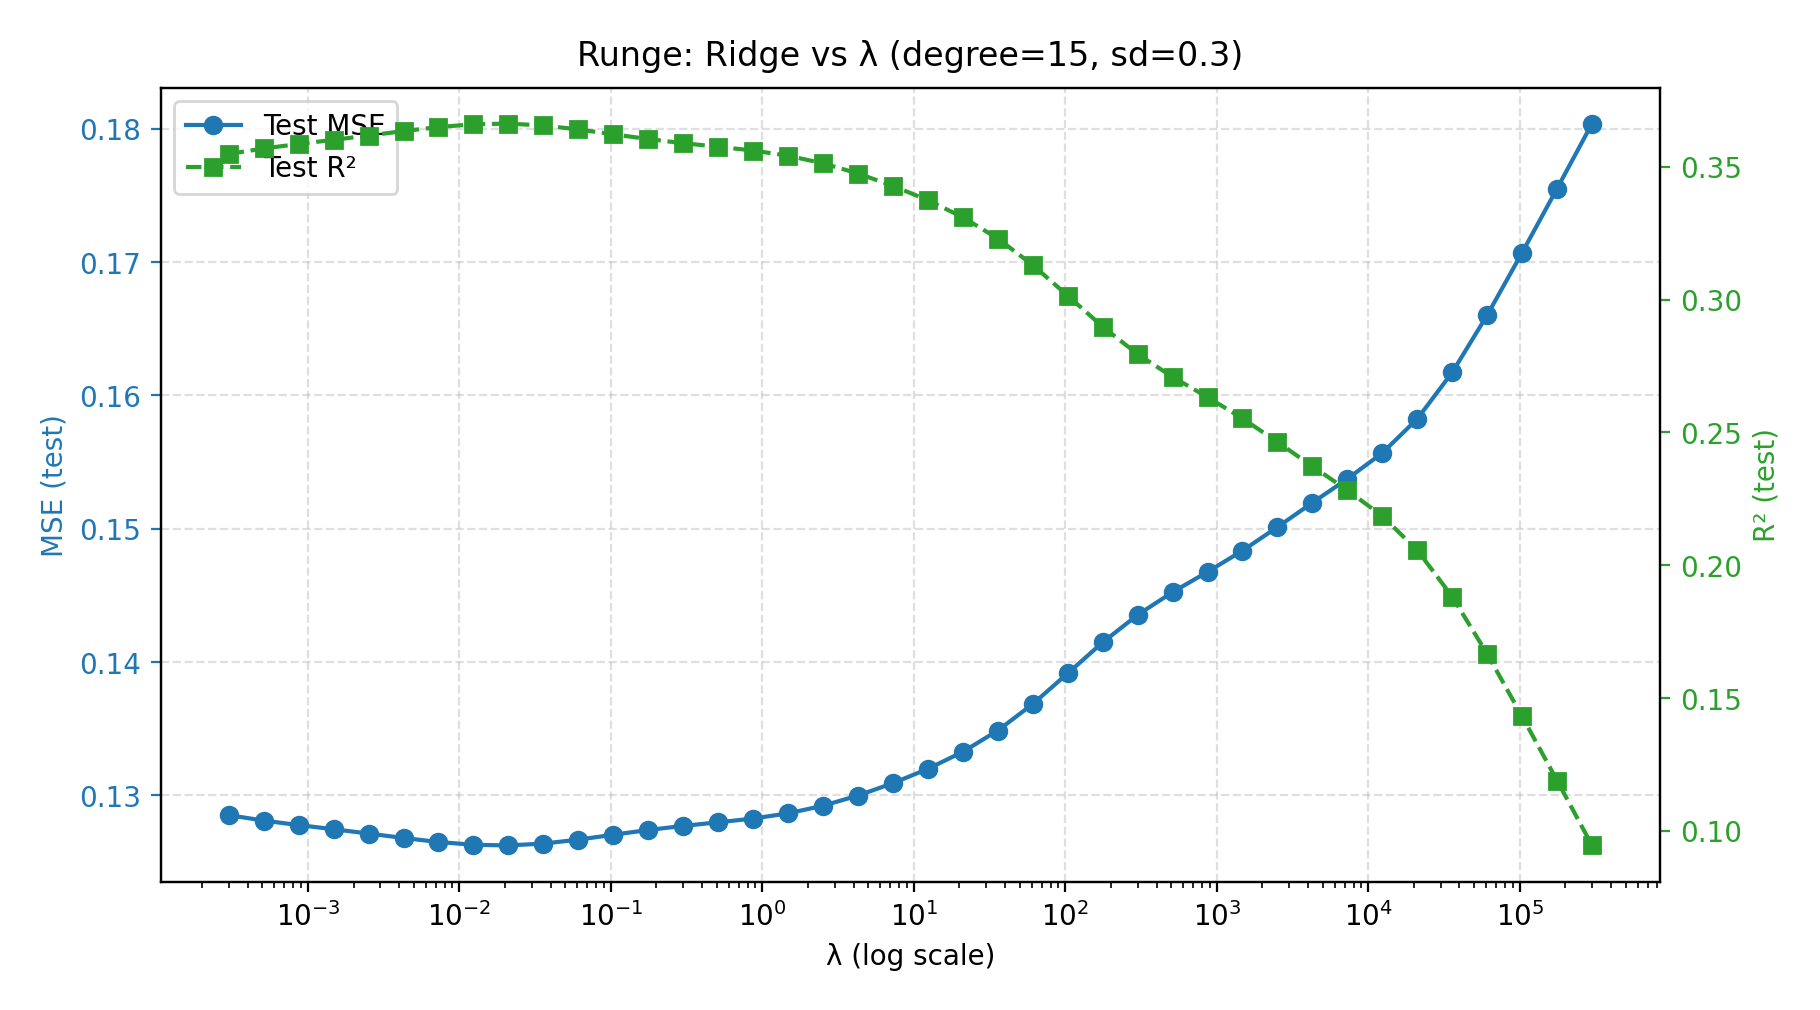
\includegraphics[width=1\linewidth]{Project-1/Figures/runge_ridge_mse_r2_vs_lambda.png}
    \caption{Test MSE and $R^2$ plotted against different $\lambda$ values.}
    \label{fig:ridge_mse_lambda}
\end{figure}

\begin{figure}[H]
    \centering
    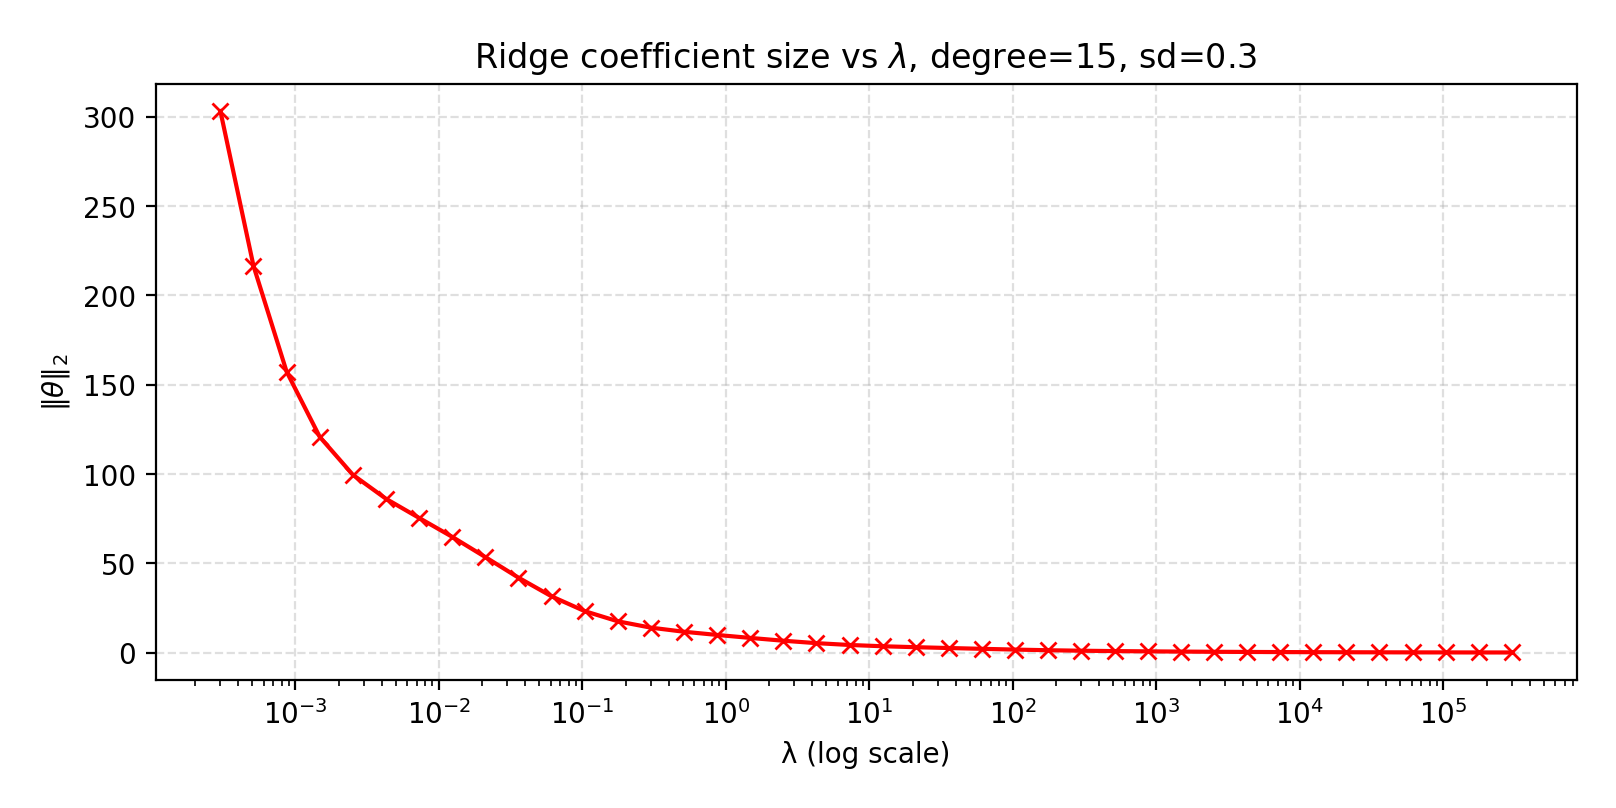
\includegraphics[width=1\linewidth]{Project-1/Figures/ridge_theta_norms_vs_lambda.png}
    \caption{The figure shows the relationshp between the $l_2$ norm of the Ridge coefficients and $\lambda$. }
    \label{fig:ridge_theta_norms}
\end{figure}

\subsubsection{Gradient descent (plain/full batch)}

From figure \ref{fig:gd_earlystop} we see that for OLS the larger $\eta$ speeds up early progress, but eventually they all approach similar loss, plateauing around 22000 iterations. For Ridge, we see the same thing, but compared to OLS fewer iterations are needed to reach the same loss, about 6800 iterations. We calculate the MSE/$R^2$ of the two GD approaches and compare to closed-form MSE/$R^2$. 

\begin{itemize}
    \item \textbf{CF OLS}\,\, \,\, \,\,\,\,  MSE= 0.1351, $R^2$ = 0.3215
    \item \textbf{GD OLS} \,\,\,\,\,\,\,\,\,   MSE= 0.1304, $R^2$ = 0.3454
    \item \textbf{CF RIDGE} \,\,  MSE= 0.1263, $R^2$ = 0.3661
    \item \textbf{GD RIDGE} \,\,  MSE= 0.1325, $R^2$ = 0.3347
\end{itemize}

We also calculate the final train loss for Ridge using CF and GD:\\ 

\textbf{TRAIN LOSS}   CF= 0.0425, GD = 0.0461



\begin{figure}[H]
    \centering
    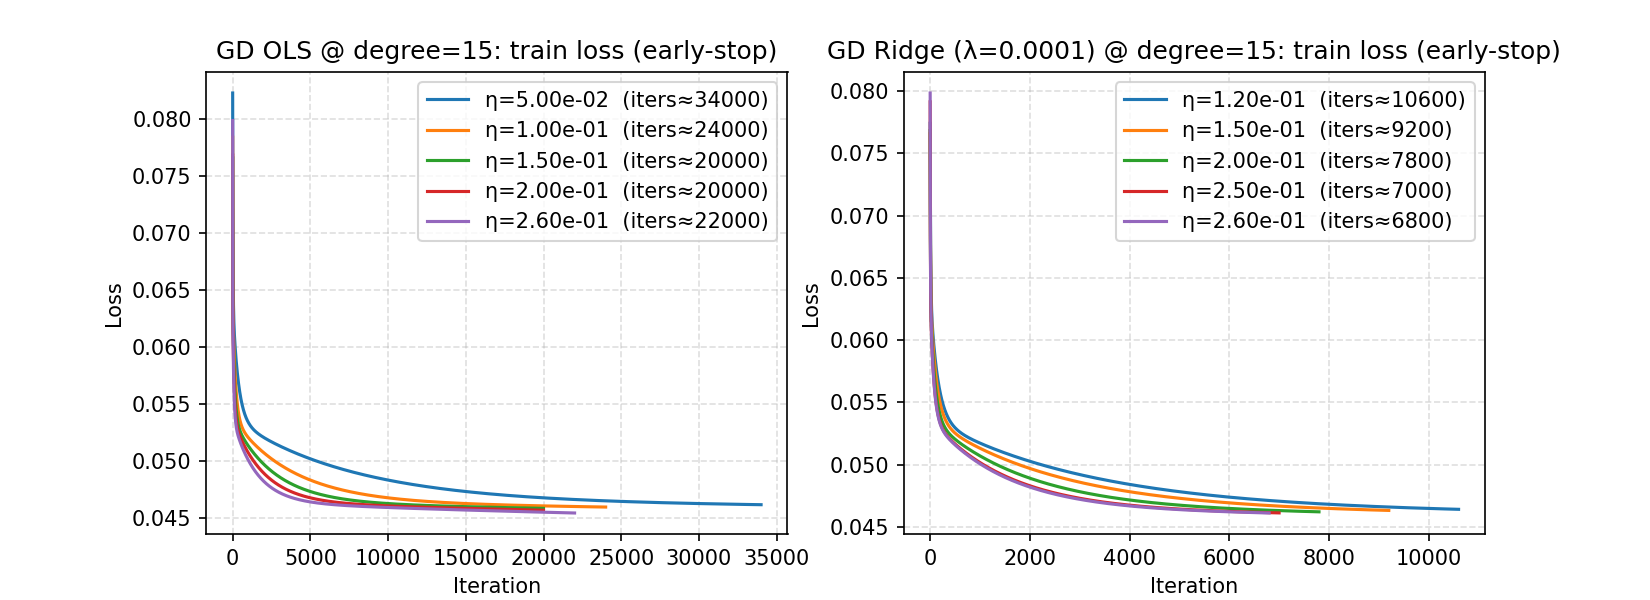
\includegraphics[width=1\linewidth]{Project-1/Figures/gd_earlystop_ols_ridge.png}
    \caption{The figure shows loss convergence curves for GD approach to OLS and Ridge for different $\eta$ steps.}
    \label{fig:gd_earlystop}
\end{figure}

\subsection{Discussion}

For the closed-form Ordinary Least Squares (OLS) method, these two curves reproduce the expected bias-variance trade-off. Increasing p reduces bias, but beyond a point the variance dominates, so test error stops improving and gets worse. In figure \ref{fig:ols_vs_degree} we see that a noiseless prediction function behaves well at higher polynomial degrees. This is a pure bias regime, with noiseless data higher-degree polynomials approximate the Runge curve better. But for the model with heavy noise we see the more characteristic U-shape we predicted in the method section, meaning that our model gives the best predictions at medium complexity and becomes unstable at higher and lower degrees.

In figure \ref{fig:norms_vs_degree} we see the ill-conditioning of high-complexity design matrices using the OLS method. Large coefficients are a classic overfitting sign, which is why we move forward to testing the Ridge method with its penalty term. \\

Ridge with its penalty term trades variance for bias. At small $\lambda$ we have low bias and higher variance, and this is where the model performs best on this split with p = 15. As we increase the penalty term, the coefficients are strongly shrunk and variance falls, but bias grows so test MSE and $R^2$ worsens. The curve for test MSE in \ref{fig:ridge_mse_lambda} is mostly monotone after its minimum at $10^{-4}-10^{-5}$, further shrinking the coefficients after this will add bias. \\

Next we replaced the analytical solution that we used for the closed-form OLS and Ridge, with a plain gradient descent with a fixed learning rate. We still used the same data, with the same noise, same polynomial degree p = 15 and the same penalty term we found worked well for the Ridge method earlier. For Ridge in GD form we still use the $\alpha$-form, as in $\alpha=\frac{\lambda}{n}$. In figure \ref{fig:} we have swept over several $\eta$ values and plotted the training loss vs iterations. For OLS, the curves descend slowly, and for Ridge they descend faster, both flattening eventually. We also printed the train loss for CF and GD; we see they don't match (as they should, meaning that GD has converged completely). We might need millions of steps to make GD converge, as GD is slow on ill-conditioned problems like high-degree Runge polynomials. Fixed step GD contracts the error p slowly, even with a well chosen $\eta$. Increasing $\lambda$ improves conditioning and speeds the convergence (with $\lambda$ = 30, we reach a plateau at many less iterations). Decreasing the tolerance or increasing the iterations also help narrowing the gap between CF and GD train loss. \\



\begin{figure}[H]
    \centering
    \includegraphics[width=1\linewidth]{Project-1/Figures/.png}
    \caption{}
    \label{fig:}
\end{figure}




\section{Conclusion}\label{section:conclusion} 

For low-noise cases and low to medium complexity, OLS works best. When introducing Ridge, we see a useful operating range of around $10^{-4}$ for this exact data, split and degree, where Ridge matches OLS but keeps coefficients smaller. However, too little shrinkage gives too large coefficients, and too much shrinkage underfits (high MSE and low $R^2$). Overall, Ridge stabilizes the degree 15 polynomial and offers a controllable bias-variance trade-off. Plain GD with a fixed learning rate works but is computationally inefficient for high degree polynomials. The learning rate $\eta$ matters, but higher $\eta$ means more progress per step, but limits speed. 

\begin{figure}[H]
    \centering
    \includegraphics[width=1\linewidth]{Project-1/Figures/.png}
    \caption{}
    \label{fig:}
\end{figure}

\bibliography{biblio}

\end{document}
